\documentclass[14pt, a4paper]{article}
\usepackage[14pt]{extsizes}




%%%%%%%%%% Математика %%%%%%%%%%
\usepackage{amsmath,amsfonts,amssymb,amsthm,mathtools}
%\mathtoolsset{showonlyrefs=true}  % Показывать номера только у тех формул, на которые есть \eqref{} в тексте.
%\usepackage{leqno} % Нумерация формул слева


%%%%%%%%%%%%%%%%%%%%%%%% Шрифты %%%%%%%%%%%%%%%%%%%%%%%%%%%%%%%%%
\usepackage{fontspec}         % пакет для подгрузки шрифтов
\setmainfont{Arial}   % задаёт основной шрифт документа

% Команда, которая нужна для корректного отображения длинных тире и некоторых других символов.
\defaultfontfeatures{Mapping=tex-text}

% why do we need \newfontfamily:
% http://tex.stackexchange.com/questions/91507/
\newfontfamily{\cyrillicfonttt}{Arial}
\newfontfamily{\cyrillicfont}{Arial}
\newfontfamily{\cyrillicfontsf}{Arial}

\usepackage{unicode-math}     % пакет для установки математического шрифта
\setmathfont{Asana Math}      % шрифт для математики
% \setmathfont[math-style=ISO]{Asana Math}
% Можно делать смену начертания с помощью разных стилей



\usepackage{polyglossia}      % Пакет, который позволяет подгружать русские буквы
\setdefaultlanguage{russian}  % Основной язык документа
\setotherlanguage{english}    % Второстепенный язык документа


%%%%%%%%%% Работа с картинками %%%%%%%%%
\usepackage{graphicx}                % Для вставки рисунков
\usepackage{graphics}
\graphicspath{{images/}{pictures/}}    % можно указать папки с картинками
\usepackage{wrapfig}                   % Обтекание рисунков и таблиц текстом




%%%%%%%%%% Графика и рисование %%%%%%%%%%
\usepackage{tikz, pgfplots}  % язык для рисования графики из latex'a


%%%%%%%%%% Гиперссылки %%%%%%%%%%
\usepackage{xcolor}              % разные цвета



\usepackage{hyperref}

\hypersetup{
    unicode=true,           % позволяет использовать юникодные символы
    colorlinks=true,       	% true - цветные ссылки, false - ссылки в рамках
    urlcolor=blue,          % цвет ссылки на url
    linkcolor=red,          % внутренние ссылки
    citecolor=green,        % на библиографию
	pdfnewwindow=true,      % при щелчке в pdf на ссылку откроется новый pdf
	breaklinks              % если ссылка не умещается в одну строку, разбивать ли ее на две части?
}

\usepackage{csquotes}            % Еще инструменты для ссылок


%%%%%%%%%% Другие приятные пакеты %%%%%%%%%
\usepackage{multicol}       % несколько колонок
\usepackage{verbatim}       % для многострочных комментариев


% Разные мелочи для русского языка из пакета babel
\setkeys{russian}{babelshorthands=true}
\usepackage{etoolbox} 


\usepackage{tikz}
\usetikzlibrary{calc}
\usetikzlibrary{decorations.pathmorphing}

\usepackage{pagecolor,lipsum}
\usepackage{titlesec}  
\usepackage{pgf,tikz}
\usepackage{mathrsfs}
\usetikzlibrary{arrows}

\newcommand{\newsize}[2]
{{\fontsize{#1}{1}\selectfont #2 }}
 \usepackage{caption}

\usepackage{fancyhdr} % Колонтитулы
\pagestyle{fancy}
\renewcommand{\headrulewidth}{0.2pt}  % Толщина линий, отчеркивающих верхний 

      
\usepackage{setspace}
\setstretch{1}  % Межстрочный интервал
\setlength{\parskip}{4mm}   % Расстояние между абзацами


\DeclareGraphicsExtensions{.pdf,.png,.jpeg,.jpg}

\usepackage[paper=a4paper,top=10mm, bottom=10mm,left=35mm,right=35mm,includefoot,includehead]{geometry}

%\newcounter{i}
%\newcommand{\pril}[1]{
%\addtocounter{i}{1} 
%Приложение \Asbuk{i}: #1}

\def\P{\tikz[remember picture,overlay] \node[opacity=0.7,inner sep=0pt] at (current page.center){
\includegraphics[width=1.2\paperwidth,height=\paperheight]{5pic}};}

\titlespacing{\section}{0pt}{-30pt}{15pt}  
\titleformat{\section} {\Large\bfseries} {Приложение \Asbuk{section}:}{7pt} {} 
\renewcommand{\sectionmark}[1]{\markright{%
\MakeUppercase{Приложение \Asbuk{section} \hspace{2mm} #1}}} 
	\lhead{\rightmark}
	\rhead{\thepage} % номер страницы
	\cfoot{Школа Чародейства и Волшебства <<Хогвартс>>}

\begin{document} % конец преамбулы, начало документа
\begin{titlepage}
\P
\center {
\includegraphics[width=6cm]{123.png}}\\
\vspace{1cm}
\flushleft \newsize{12}{Мистеру Поттеру}
\\
\vspace{2.5cm}
Дорогая Дарья Лобачёва,

Мы рады проинформировать вас , что вам представлено место в Школе Чародейства и Волшебства "Хогвартс"

Пожалуйста, ознакомьтесь с приложенным к данному письму списком необходимых книг и предметов.

Занятия начинаются 1 сентября. Ждём вашу сову не позднее 31 июля.

Искренне ваша,\\
Minerva Mc Gonagall\\
\newsize{28}{\fontspec{Benvolio Font4You}{Minerva Mc Gonagall}}\\
заместитель директора 
\vfill
\center{Школа Чародейства и Волшебства <<Хогвардс>>\\\newsize{12}{Директор: Альбус Дамблдор\\ (Кавалер ордена Мерлина первой степени, основатель ордена Феникса, председатель Международной КонференцииМагов)}}\\
\href{https://www.wbstudiotour.co.uk/}{Школа Хогвартс}
\clearpage
\end{titlepage}
\newpage
\P
\section{Список необходимых книг и предметов}
\newcommand*{\MyPoint}{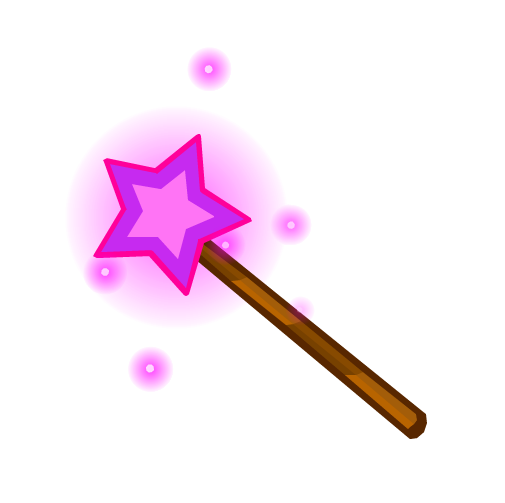
\includegraphics[scale=0.05]{234.png}}
\renewcommand{\labelitemi}{\MyPoint}
\begin{itemize}
\item Волшебная палочка
\item Мантия-неведимка
\item Камень оживляющий мёртвых
\item Карта Хогвартса
\item Магическое животное: сова, кот или жаба
\item Билет на поезд 
\item Три простых рабочих мантии (черных)
\item Котел (оловянный, стандартный размер №2)
\item Комплект стеклянных или хрустальных флаконов
\item Телескоп
\item Медные весы
\end{itemize}
\newpage
\P
\section{Список изучаемых предметов}
\newcommand*{\MePoint}{
\includegraphics[scale=0.1]{halloween_hat-5.png}}
\renewcommand{\labelitemi}{\MePoint}
\begin{itemize}
\item Заговоры и заклинания
\item История магии
\item Теория магии
\item Трансфигурация
\item Магическая травология
\item Магические отвары и зелья
\item Зоология:фантастические твари
\item Темные силы: пособие по самозащите
\end{itemize}


\end{document}